\anonsection{Цель лабораторной работы}
Целью лабораторной работы №1 является освоение возможностей программы Microsoft Project для планирования проекта по разработке программного обеспечения.
Каждое задание лабораторной работы №1 должно выполняться и сохраняться в отдельном файле MS Project.

Команда разработчиков из 16 человек занимается созданием карты города на основе собственного модуля отображения. 
Проект должен быть завершен в течение 6 месяцев. Бюджет проекта: 50 000 рублей

\anonsection{Тренировочное задание}
Вариант по Электронному Университету -- 4, следовательно, для тренировочного задания выбран вариант 0.

Требуется выполнить планирование тестового проекта в соответствии с методическим пособием.
Результат представлен на рисунке 1:
\FloatBarrier
\begin{figure}[h]	
	\begin{center}
		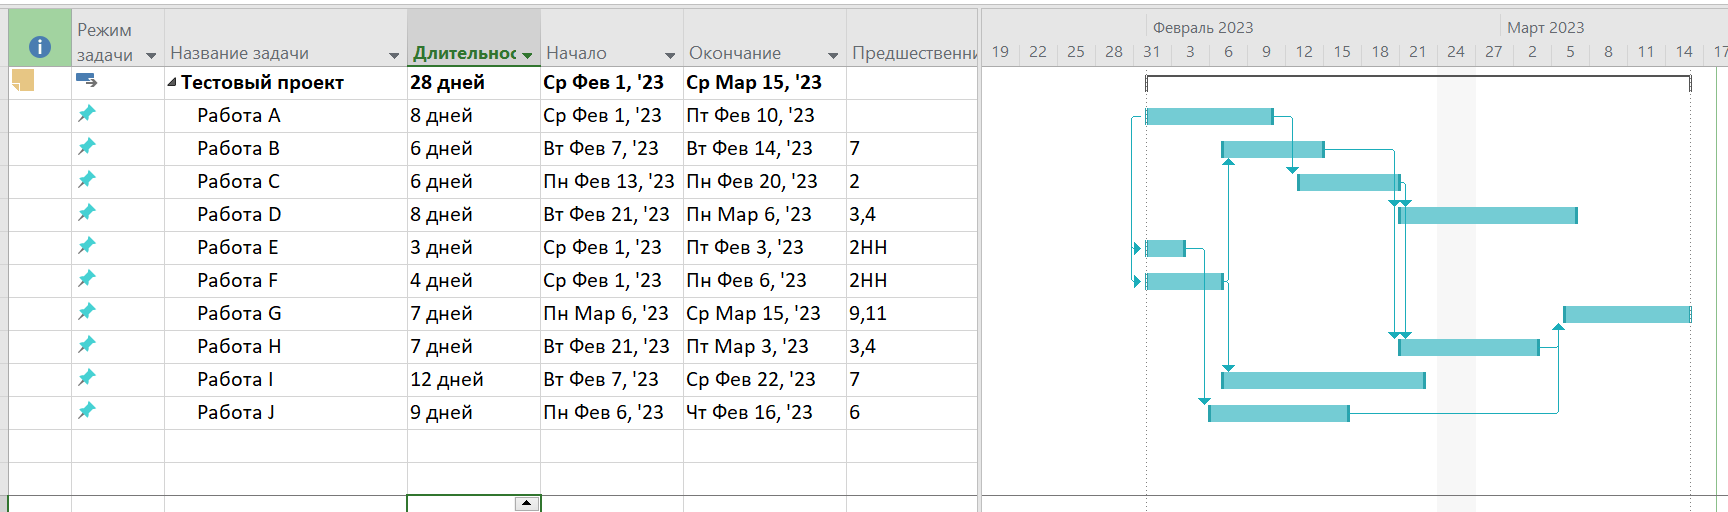
\includegraphics[width=\linewidth]{inc/test.png}
	\end{center}
	\captionsetup{justification=centering}
	\caption{Выполнение тестового задания}
\end{figure}
\FloatBarrier


\newpage
\anonsection{Задание 1}
В этом задании требуется настроить рабочую среду проекта.

Лабораторная работа выполнена в Microsoft Project 2016 года, операционная система -- Windows 7, запущенная на виртуальной машине.

\subsection*{Основная настройка проекта}
Во вкладке \textit{Проект} -> \textit{Основные настройки проекта} была установлена дата начала проекта и стандартный календарь.

\FloatBarrier
\begin{figure}[h]	
	\begin{center}
		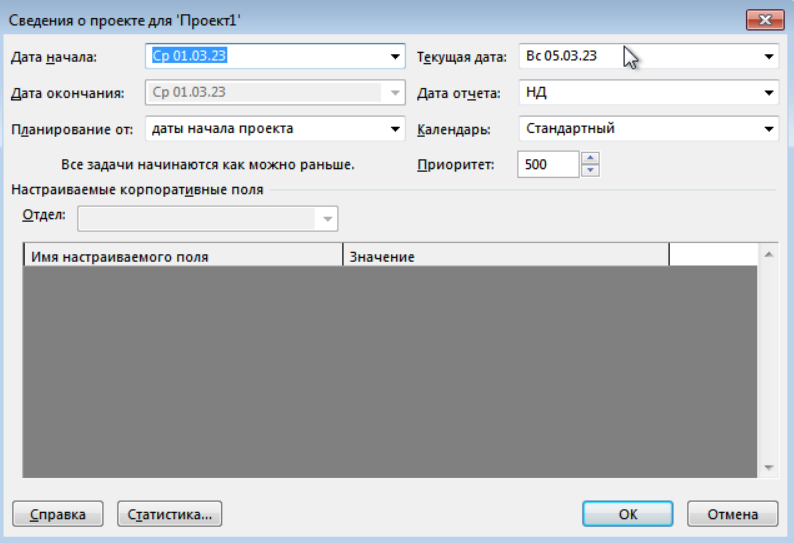
\includegraphics[width=\linewidth]{inc/1-1.png}
	\end{center}
	\captionsetup{justification=centering}
	\caption{Выполнение подпунктов 1 и 6}
\end{figure}
\FloatBarrier

\newpage
Во вкладке \textit{Файл} -> \textit{Параметры} были указаны следующие параметры для проекта:
\begin{enumerate}
	\item Длительность работы -- в неделях, тип работ -- с фиксированными трудозатратами;
	\item 8 рабочих часов в день, 40 рабочих часов в неделю;
	\item Начало рабочей недели -- в понедельник, начало финансового года -- с января;
	\item Продолжительность рабочего дня -- с 9 часов до 18.
\end{enumerate}

\FloatBarrier
\begin{figure}[h]	
	\begin{center}
		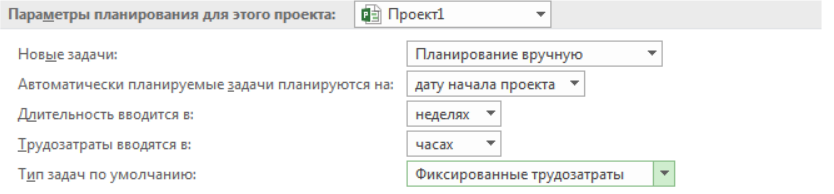
\includegraphics[width=\linewidth]{inc/1-2.png}
	\end{center}
	\captionsetup{justification=centering}
	\caption{Выполнение подпункта 2}
\end{figure}
\FloatBarrier

\FloatBarrier
\begin{figure}[h]	
	\begin{center}
		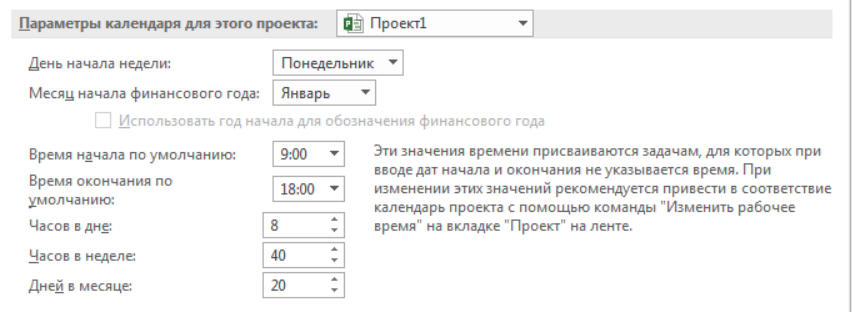
\includegraphics[width=\linewidth]{inc/1-3.png}
	\end{center}
	\captionsetup{justification=centering}
	\caption{Выполнение подпунктов 3-5}
\end{figure}
\FloatBarrier


\subsection*{Настройка выходных и праздничных дней}
Во вкладке \textit{Проект} -> \textit{Свойства} -> \textit{Изменение рабочего проекта} можно посмотреть текущий календарь проекта.

Так как календарь выбран стандартным, а начало рабочего дня -- с понедельника, то выходные уже проставлены автоматически, поэтому требуется только настроить праздничные дни под российский календарь.

Все праздники в 2023 году были проставлены в исключения для календаря, дни указаны на графике как праздничные.
Для каждого государственного праздника выставлены дни, указанные в официальном календаре на 2023 год. 
Например, нерабочие дни из-за Дня России указаны с 10 по 12 июня, несмотря на то, что 10 и 11 числа -- выходные.

\FloatBarrier
\begin{figure}[h]	
	\begin{center}
		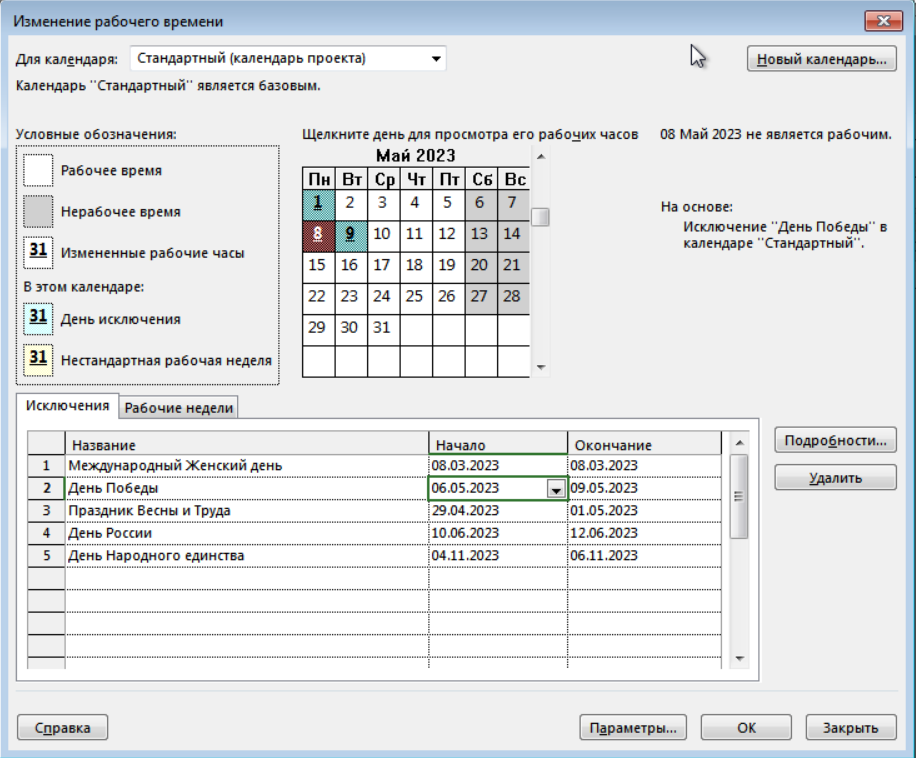
\includegraphics[width=\linewidth]{inc/1-7.png}
	\end{center}
	\captionsetup{justification=centering}
	\caption{Выполнение подпункта 7}
\end{figure}
\FloatBarrier

\subsection*{Суммарная задача проекта и заметки}
Для добавления суммарной задачи проекта использовалась вкладка \textit{Задача} -> \textit{Вставить} -> \textit{Вставить суммарную задачу проекта}.

В качестве дня завершения было выбрано 1 сентября, так как по условию лабораторной работы на проект выделено полгода.

Результат представлен на рисунке 6:
\FloatBarrier
\begin{figure}[h]	
	\begin{center}
		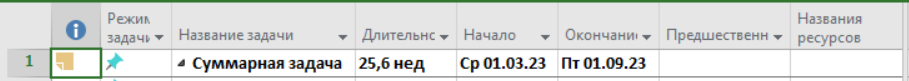
\includegraphics[width=\linewidth]{inc/1-81.png}
	\end{center}
	\captionsetup{justification=centering}
	\caption{Выполнение подпункта 8}
\end{figure}
\FloatBarrier

Заметка была прикреплена к суммарной задаче проекта, её можно прочитать, наведя на иконку на первом столбце в строке с суммарной задачей проекта.
\FloatBarrier
\begin{figure}[h]	
	\begin{center}
		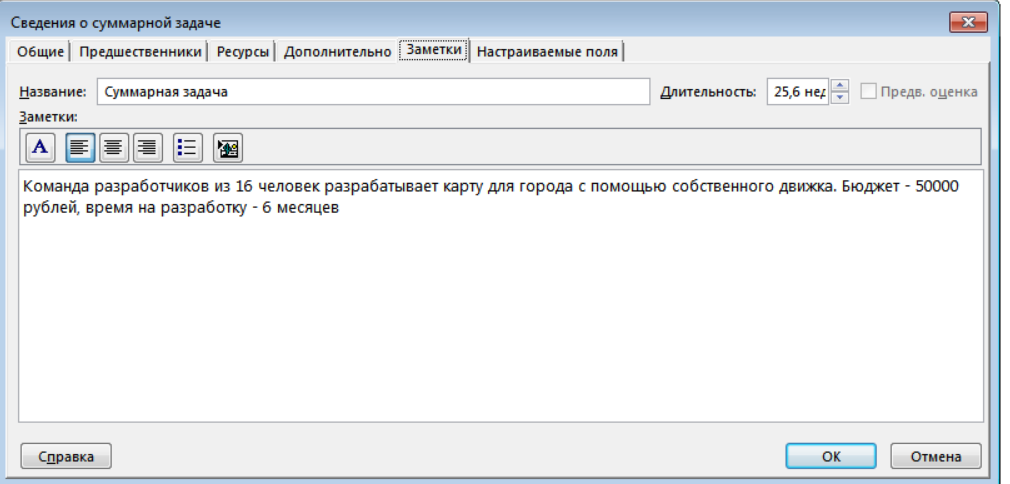
\includegraphics[width=\linewidth]{inc/1-82.png}
	\end{center}
	\captionsetup{justification=centering}
	\caption{Выполнение подпункта 8 (заметки)}
\end{figure}
\FloatBarrier

Итоговый результат был сохранен в отдельном файле \textit{task1.mpp}.

\anonsection{Задание 2}
Требуется ввести все задачи в соответствии с таблицей, приведенной в задании к лабораторной работе.

Для добавлении задачи использовалась вкладка \textit{Задача} -> \textit{Вставить} -> \textit{Вставить задачу}.
Для добавления вех использовалась вкладка \textit{Задача} -> \textit{Вставить} -> \textit{Вставить веху}.
Отличие вех от задач состоит в том, что для вех не проставляется продолжительность.

Меню добавления задачи представлена на рисунке 8:
\FloatBarrier
\begin{figure}[h]	
	\begin{center}
		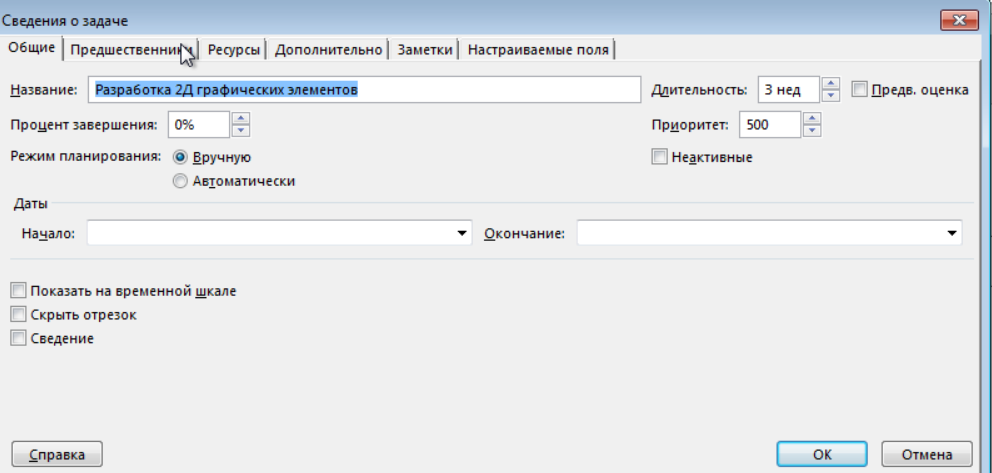
\includegraphics[width=\linewidth]{inc/2-1.png}
	\end{center}
	\captionsetup{justification=centering}
	\caption{Добавление новой задачи}
\end{figure}
\FloatBarrier

\newpage

Итоговый результат представлен на рисунке 9:
\FloatBarrier
\begin{figure}[h]	
	\begin{center}
		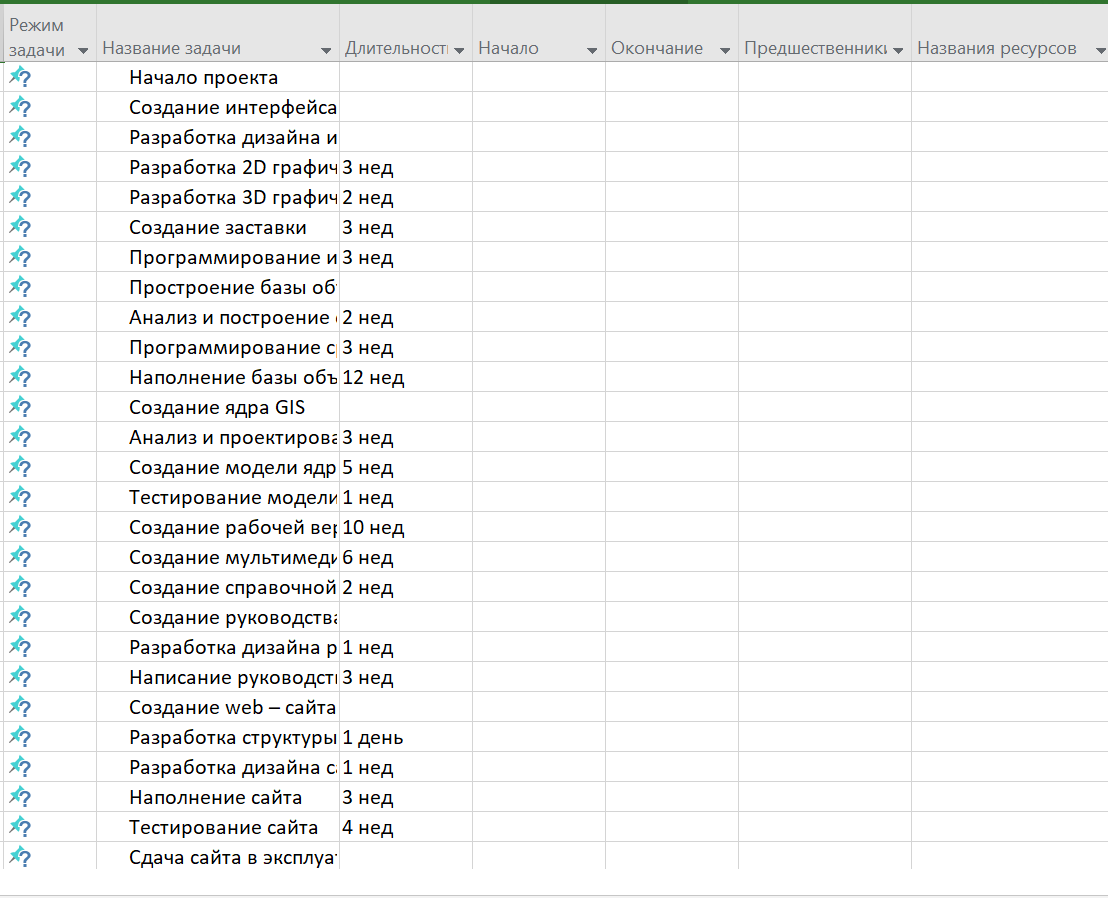
\includegraphics[height=18cm, width=\linewidth]{inc/tasks.png}
	\end{center}
	\captionsetup{justification=centering}
	\caption{Выполнение задания 2}
\end{figure}
\FloatBarrier

Получившаяся программа была сохранена в отдельном файле \textit{task2.mpp}.

\anonsection{Задание 3}
Требуется сгруппировать список задач в соответствии с требованиями, указанными в лабораторной работе.
Для изменения вложенности задач использовались вкладки в меню, приведенные на рисунке 10:
\FloatBarrier
\begin{figure}[h]	
	\begin{center}
		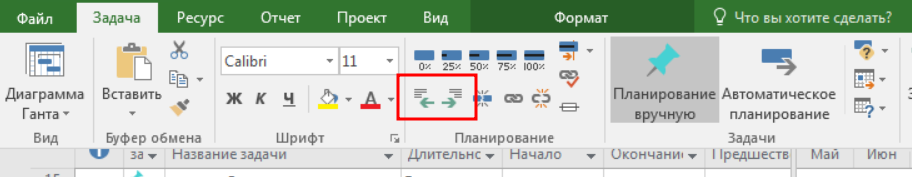
\includegraphics[width=\linewidth]{inc/3-3.png}
	\end{center}
	\captionsetup{justification=centering}
	\caption{Добавление новой задачи}
\end{figure}
\FloatBarrier

Получившаяся программа была сохранена в отдельном файле \textit{task3.mpp}. 
Из-за того, что в первом задании была добавлена суммарная задача проекта, индексы по сравнению с таблицей из ТЗ сдвинуты на 1.

Итоговый результат представлен на рисунке 11:
\FloatBarrier
\begin{figure}[h]	
	\begin{center}
		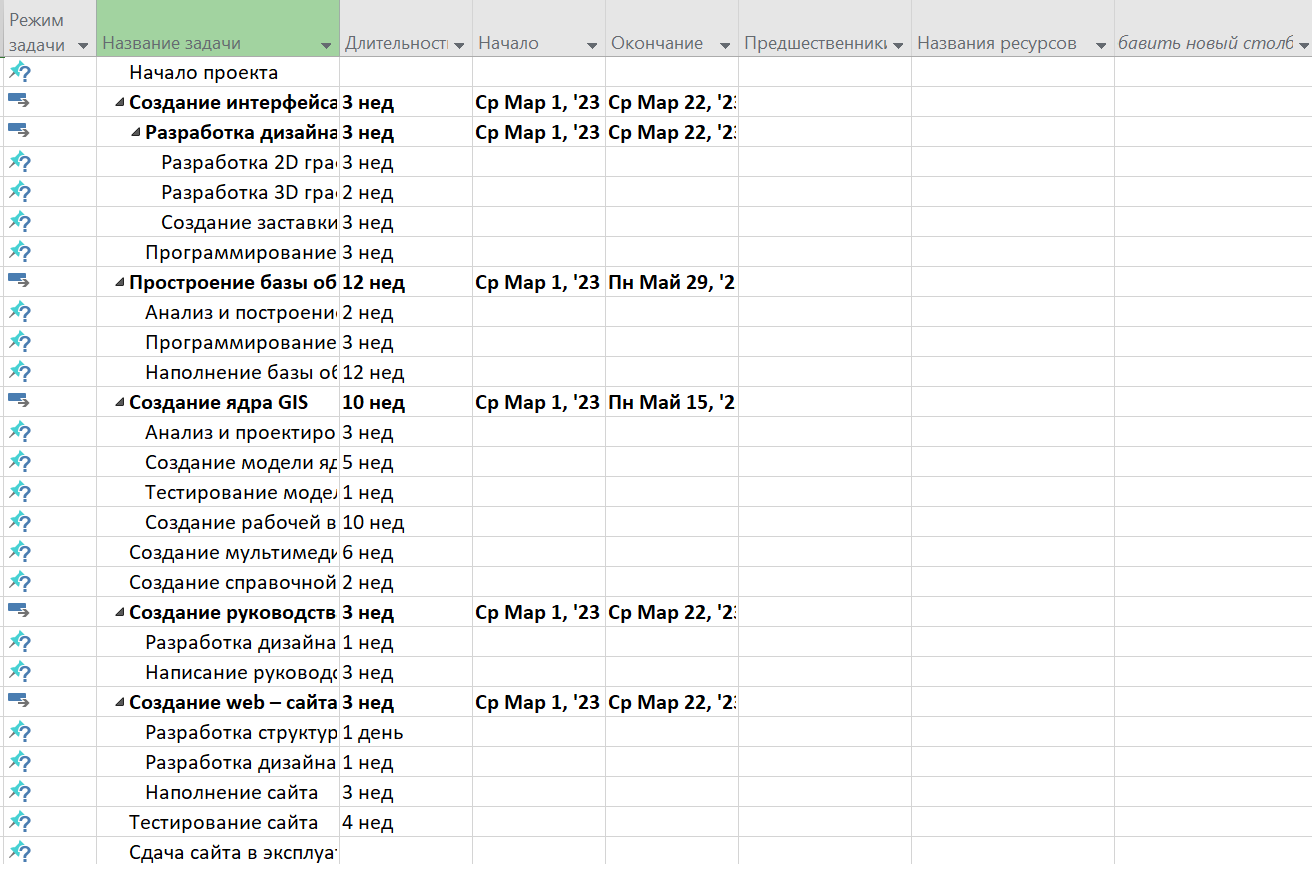
\includegraphics[width=\linewidth]{inc/tasks1.png}
	\end{center}
	\captionsetup{justification=centering}
	\caption{Выполнение задания 3}
\end{figure}
\FloatBarrier

\anonsection{Задание 4}
Требуется установить связи между задачами в соответствии с требованиями, указанными в лабораторной работе.

Для создания связи между двумя задачами требовалось выделить с одновременным нажатием клавиши CTRL все требуемые задачи, а затем выбрать пункт \textit{Связать задачи}.

По умолчанию задачи связываются между собой типом <<Окончание-Начало>>, что соответствует тому, что задача начнется только после завершения предыдущей. 
По двойному нажатию на задачу откроется меню задачи, где можно выбрать другой тип связи, а также указать задержку, если такая существует.

На рисунке 12 показано меню, в котором можно настроить тип связи между задачами и указать задержку:
\FloatBarrier
\begin{figure}[h]	
	\begin{center}
		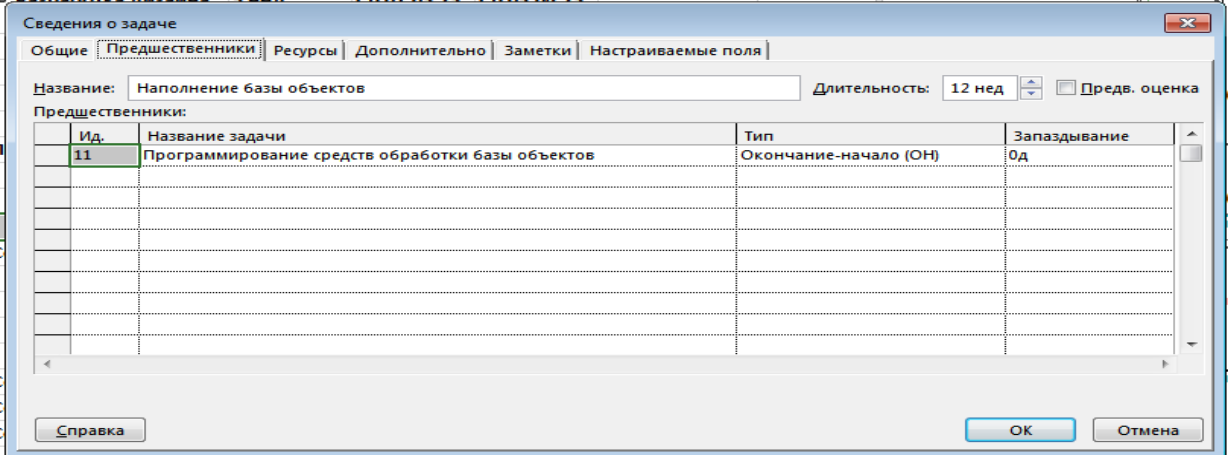
\includegraphics[width=\linewidth]{inc/4-1.png}
	\end{center}
	\captionsetup{justification=centering}
	\caption{Меню изменения связи между задачами}
\end{figure}
\FloatBarrier


\newpage
Получившаяся программа была сохранена в отдельном файле \textit{task4.mpp}.

Итоговый результат представлен на рисунке 13:
\FloatBarrier
\begin{figure}[h]	
	\begin{center}
		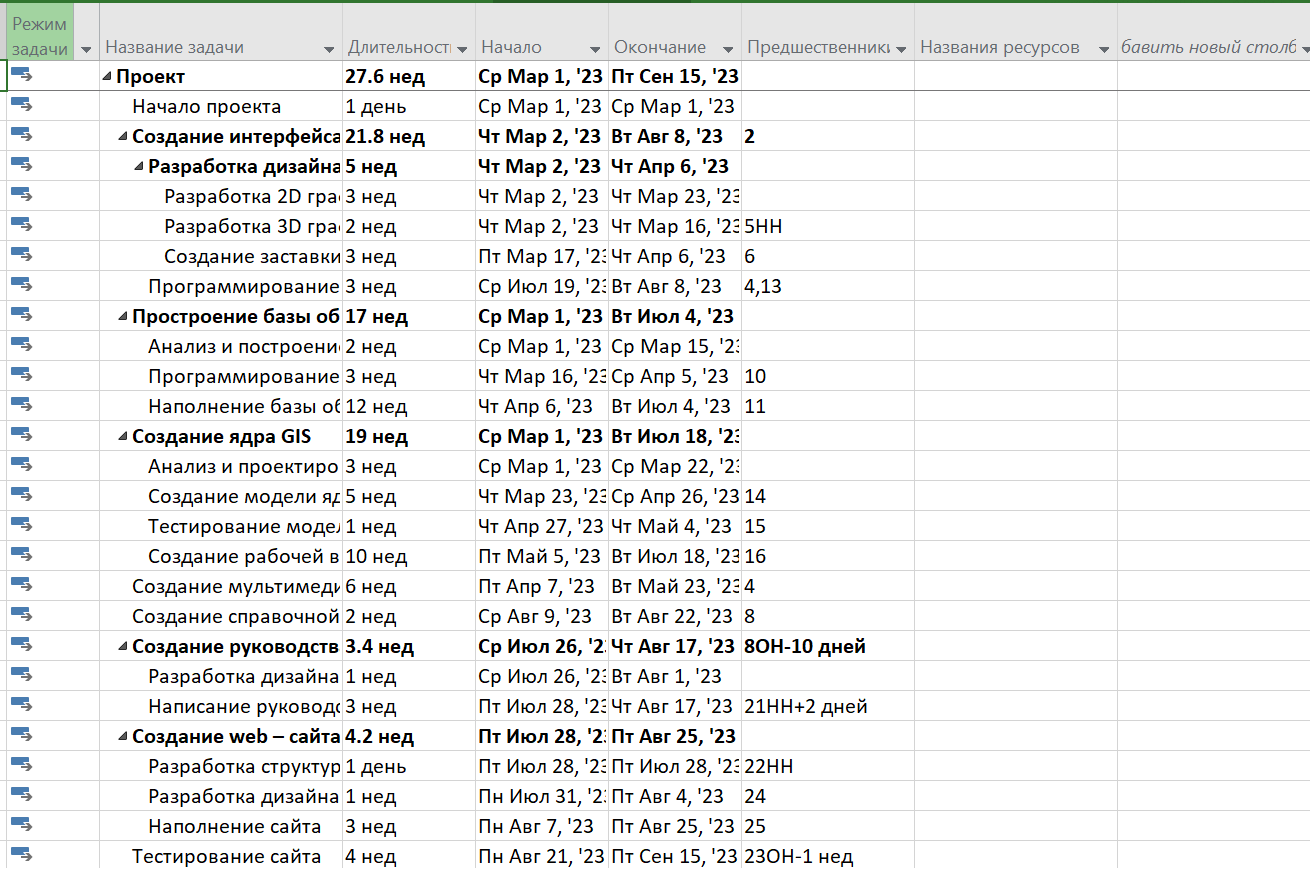
\includegraphics[width=\linewidth, height=9.5cm]{inc/result.png}
	\end{center}
	\captionsetup{justification=centering}
	\caption{Выполнение задания 4}
\end{figure}
\FloatBarrier

\anonsection{Выводы}
В результате выполнения лабораторной работы удалось построить таблицу задач, требуемых для реализации проекта.

В текущем виде проект, если строго держаться плана и учитывать календарь, удастся выполнить только к 15 сентября, что чуть больше, чем полгода, выделенных на реализацию проекта. 
Тем не менее, к 1 сентября будут выполнены все этапы, кроме тестирования, соответственно, программное обеспечение будет уже к этому времени разработано, хоть и не до конца протестировано.

С самого начала работы проекта можно параллельно заниматься созданием интерфейса, построением базы объектов и созданием ядра GIS.
Создание руководства пользователя и создание сайта требуют выполнения предыдущих задач, поэтому эти действия по плану начнутся значительно позже -- 26 июля, то есть спустя 4.5 месяца после запуска проекта.

Самый продолжительный этап -- создание интерфейса. Несмотря на то, что по отдельности этапы занимают небольшое время, они требует выполнения предыдущих задач, из-за чего все растягивается.

По итогам лабораторной работы удалось также познакомиться с возможностями программы Microsoft Project.